
\begin{frame}{Spot Lights - Introduction}
  \begin{columns}
    \begin{column}{0.7\textwidth}
      \begin{raybox}{Spot Light Characteristics}
        Light emanating from a point within a cone

        \only<2>{
          \vspace{0.1cm}
          \textbf{Real-world examples:}
          \begin{itemize}
            \item Flashlights, headlights
            \item Stage spotlights
            \item Desk lamps
          \end{itemize}
        }
      \end{raybox}

      \only<3>{
        \begin{center}
          \begin{figure}
            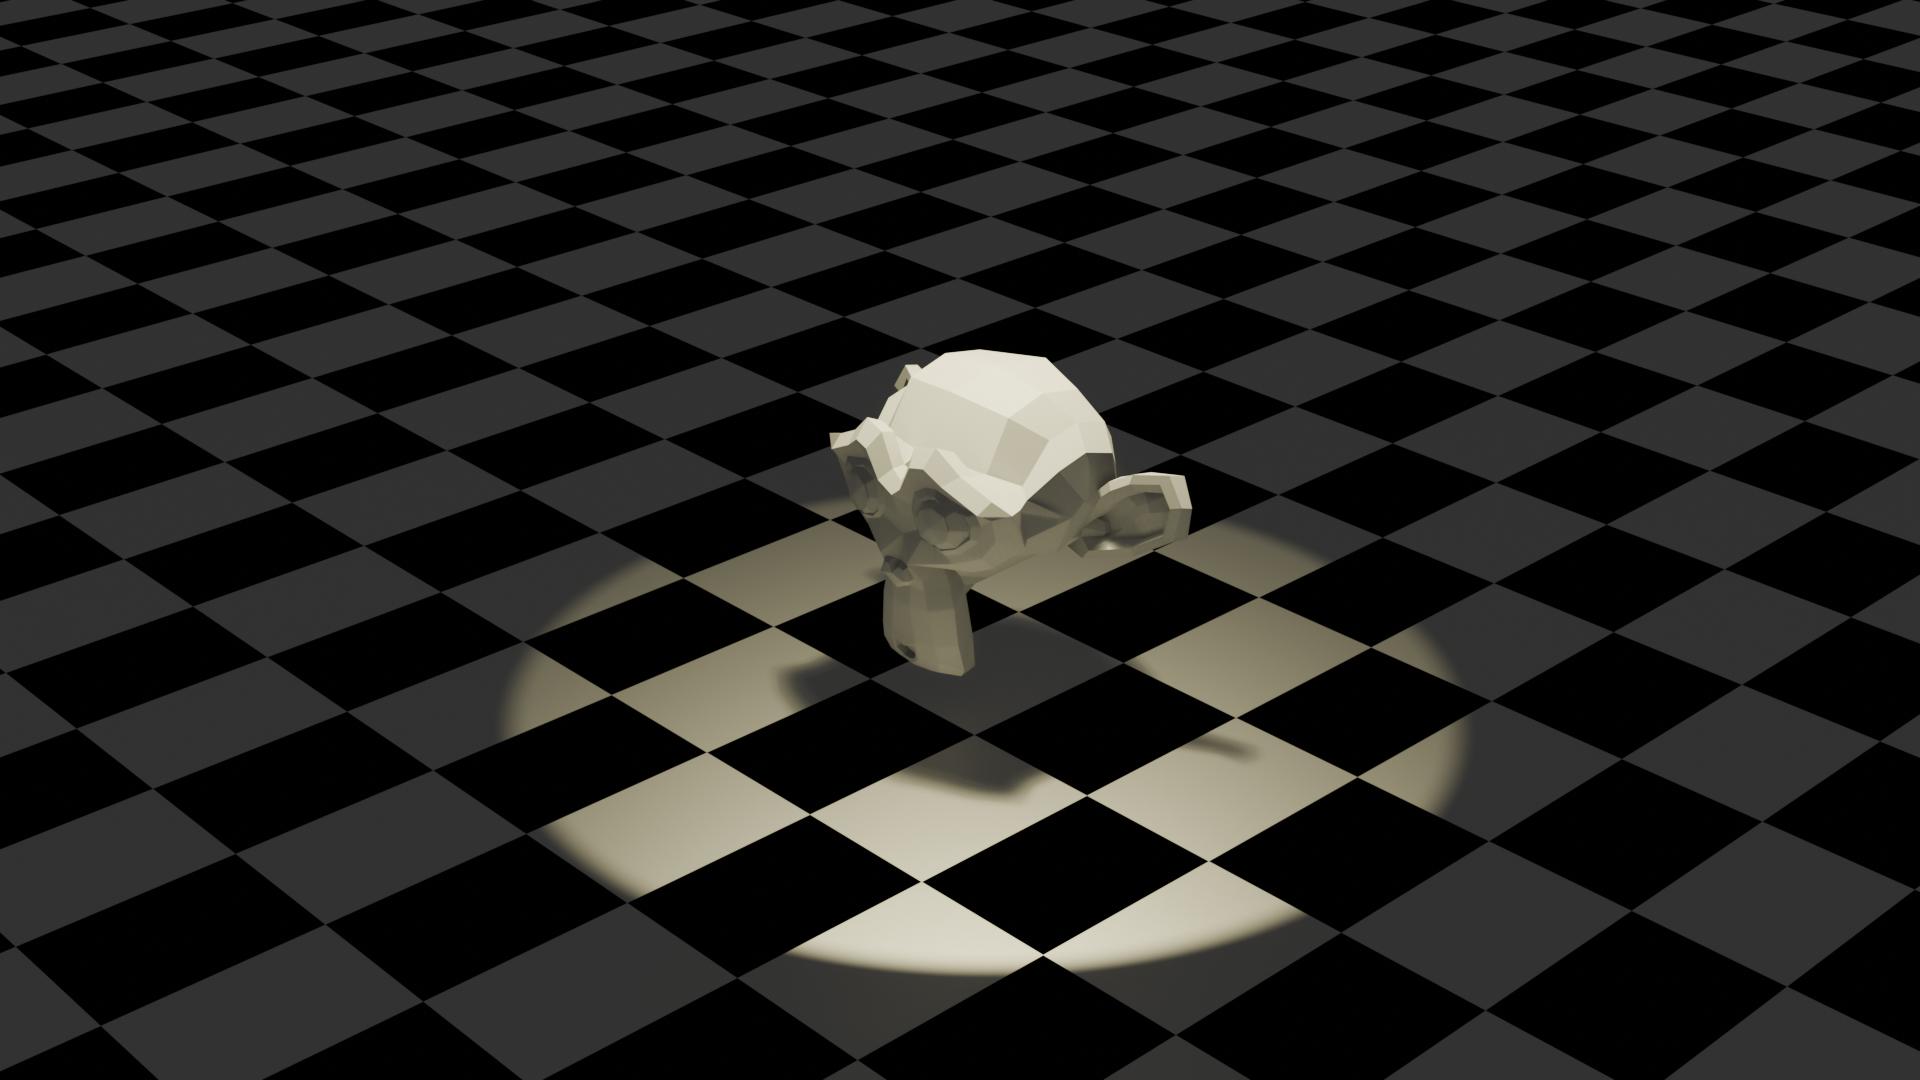
\includegraphics[width=\linewidth]{images/spot.png}
            \caption{Spot Light ft. Suzanne the monkey}
          \end{figure}
        \end{center}
      }
    \end{column}
    \begin{column}{0.3\textwidth}
      \centering
      \begin{tikzpicture}[scale=0.8]
        \node[circle, fill=LightColor, minimum size=0.6cm] (light) at (1,3) {\footnotesize S};
        \node[above] at (1,3.5) {\footnotesize Spotlight};

        \draw[lightray, thick] (light) -- (0,0);
        \draw[lightray, thick] (light) -- (2,0);
        \draw[lightray, fill=LightColor, opacity=0.2] (light) -- (0,0) -- (2,0) -- cycle;

        \draw[->, red, very thick] (light) -- (1,1.5);
        \node[right] at (1.2,2.2) {\footnotesize Direction};

        \draw[dashed] (light) -- (1,0);
        \node[right] at (1.5,1) {\footnotesize $\theta$};

        \node[sphere, minimum size=0.6cm] (obj1) at (0.7,-0.5) {};
        \node[sphere, minimum size=0.6cm,fill=ObjectColor!60] (obj2) at (3,-0.5) {};

        \node[below] at (0.7,-1) {\footnotesize Lit};
        \node[below] at (3,-1) {\footnotesize Dark};
      \end{tikzpicture}
    \end{column}
  \end{columns}
\end{frame}

\begin{frame}{Spot Light Mathematics - Cone Calculation}
  \begin{columns}
    \begin{column}{0.7\textwidth}
      \begin{mathbox}{Spot Light Parameters}
        \textbf{Position:} $\mathbf{P}_{\text{light}}$

        \textbf{Direction:} $\mathbf{D}_{\text{spot}}$ (where spotlight points)

        \textbf{Cone angle:} $\theta_{\text{cutoff}}$ (half-angle of cone)

        \textbf{Falloff exponent:} $e$ (controls edge softness)

        \vspace{0.3cm}
        \pause
        \textbf{Step 1 - Calculate angle to surface:}
        \begin{align*}
          \hat{\mathbf{L}} &= \frac{\mathbf{P}_{\text{light}} - \mathbf{P}_{\text{surface}}}
          {|\mathbf{P}_{\text{light}} - \mathbf{P}_{\text{surface}}|} \\
          \cos(\alpha) &=  \mathbf{D}_{\text{spot}} \cdot (- \hat{\mathbf{L}})
        \end{align*}

        \pause
        \textbf{Step 2 - Check if inside cone:}
        \begin{align}
          \text{if } \cos(\alpha) > \cos(\theta_{\text{cutoff}}) \text{ then illuminate}
        \end{align}
      \end{mathbox}
    \end{column}
    \begin{column}{0.3\textwidth}
      \begin{tikzpicture}[scale=0.8]
        % Spotlight
        \node[circle, fill=LightColor, minimum size=0.6cm] (light) at (2,3) {};

        % Spotlight direction
        \draw[->, red, very thick] (light) -- (2,1.5);
        \node[right] at (2.2,2.2) {\footnotesize $\mathbf{D}_{\text{spot}}$};

        % Surface point
        \fill[ObjectColor] (1,1) circle (3pt);
        \node[below] at (1,0.7) {\footnotesize Surface};

        % Vector to surface
        \draw[->, blue, thick] (light) -- (1,1);
        \node[left] at (1.3,2) {\footnotesize $\mathbf{L}$};

        % Angle between them
        \draw[dashed] (2,3) -- (2,1.5);
        \draw[dashed] (2,3) -- (1,1);
        \node[AccentColor] at (1.7,2.3) {\footnotesize $\alpha$};

        % Cone edges
        \draw[lightray, dashed] (light) -- (1.2,0.5);
        \draw[lightray, dashed] (light) -- (2.8,0.5);
        \node[below] at (2,0.2) {\footnotesize $\theta_{\text{cutoff}}$};
      \end{tikzpicture}
    \end{column}
  \end{columns}
\end{frame}

\begin{frame}{Spot Light Attenuation}
  \begin{mathbox}{Complete Spot Light Formula}
    \textbf{Angular attenuation:}
    \begin{align}
      \text{spot\_factor} =
      \begin{cases}
        (\cos(\alpha))^e & \text{if } \cos(\alpha) > \cos(\theta_{\text{cutoff}}) \\
        0 & \text{otherwise}
      \end{cases}
    \end{align}

    \pause
    \textbf{Distance attenuation (same as point light):}
    \begin{align}
      \text{distance\_attenuation} = \frac{1}{a + b \cdot d + c \cdot d^2}
    \end{align}

    \pause
    \textbf{Final intensity:}
    \begin{align}
      I_{\text{final}} = I_{\text{light}} \cdot \text{spot\_factor} \cdot \text{distance\_attenuation}
    \end{align}
  \end{mathbox}

  \vspace{0.3cm}
  \pause
  \begin{center}
    % IMAGE: Spotlight falloff demonstration
    % Show effect of different exponent values on spotlight edge softness
    % \includegraphics[width=0.8\linewidth]{images/spotlight_falloff.jpg}
    \textcolor{gray}{[Spotlight falloff with different exponents]}
  \end{center}
\end{frame}
